\documentclass[tikz,border=10pt]{standalone}
\usepackage{amsmath,amssymb}
\usepackage{tikz}
\usetikzlibrary{arrows,automata,backgrounds,calendar,chains,decorations,decorations.pathreplacing,decorations.text,fit,matrix,mindmap,patterns,petri,plotmarks,positioning,shadows,shapes,shapes.callouts,shapes.geometric,shapes.misc,spy,trees,calc,intersections,tikzmark,arrows.meta}
\usepackage{xcolor}
\usepackage{pgfplots}
\pgfplotsset{compat=1.16}

% Common math macros from the book
\def\x{\mathbf{x}}
\def\y{\mathbf{y}}
\def\z{\mathbf{z}}
\def\A{\mathbf{A}}
\def\b{\mathbf{b}}
\def\c{\mathbf{c}}
\def\w{\mathbf{w}}
\def\v{\mathbf{v}}
\def\u{\mathbf{u}}
\def\e{\mathbf{e}}
\def\zero{\mathbf{0}}
\def\R{\mathbb{R}}
\def\N{\mathbb{N}}
\def\Z{\mathbb{Z}}
\def\Q{\mathbb{Q}}
\def\st{\text{s.t.}}
\def\vect#1{\mathbf{#1}}
\def\xLP{x^{\mathrm{LP}}}
\def\zLP{z^{\mathrm{LP}}}
\def\xIP{x^{\mathrm{IP}}}

% Common node styles from the book
\tikzset{
    main/.style={circle, draw, fill=gray!20, minimum size=1cm, font=\normalsize},
    dot/.style={circle,fill=blue,minimum size=3pt,inner sep=0pt, outer sep=-1pt},
    vertex/.style={circle,fill=black!25,minimum size=20pt,inner sep=0pt},
    edge/.style={draw,-,thick},
    directed edge/.style={draw,->,>=latex,thick},
}

% Additional macros for 3D/coordinate systems
\newcommand{\xhat}{\hat{\x}}
\newcommand{\yhat}{\hat{\y}}
\newcommand{\zhat}{\hat{\z}}
\newcommand{\ihat}{\hat{\imath}}
\newcommand{\jhat}{\hat{\jmath}}
\newcommand{\khat}{\hat{k}}

\begin{document}
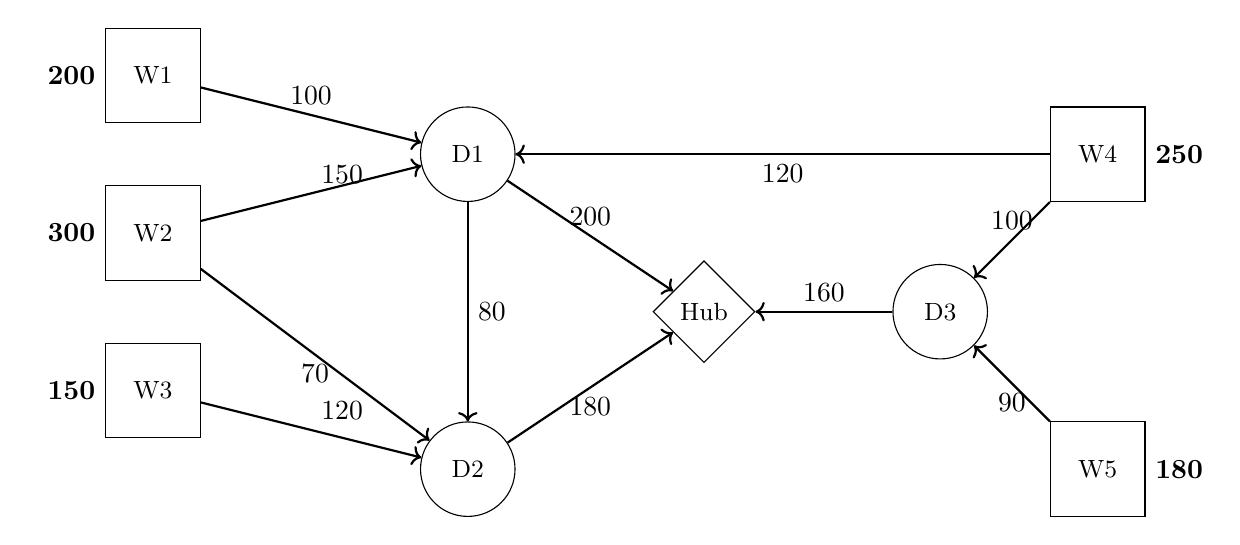
\begin{tikzpicture}[
    node distance=1.5cm and 2.5cm,
    warehouse/.style={draw, rectangle, minimum size=1.2cm, font=\small},
    distribution/.style={draw, circle, minimum size=1.2cm, font=\small},
    hub/.style={draw,  diamond, minimum size=1.2cm, font=\small}]

   % Nodes with inventory labels
    \node[warehouse, label=left:{\textbf{ 200}}] (W1) at (-4,3) {W1};
    \node[warehouse, label=left:{\textbf{300}}] (W2) at (-4,1) {W2};
    \node[warehouse, label=left:{\textbf{150}}] (W3) at (-4,-1) {W3};
    \node[distribution] (D1) at (0,2) {D1};
    \node[distribution] (D2) at (0,-2) {D2};
    \node[hub] (Hub) at (3,0) {Hub};
    \node[warehouse, label=right:{\textbf{250}}] (W4) at (8,2) {W4};
    \node[warehouse, label=right:{\textbf{180}}] (W5) at (8,-2) {W5};
    \node[distribution] (D3) at (6,0) {D3};

    % Arcs
    \draw[->, thick] (W1) -- node[above] {100} (D1);
    \draw[->, thick] (W2) -- node[above right] {150} (D1);
    \draw[->, thick] (W3) -- node[above right] {120} (D2);
    \draw[->, thick] (D1) -- node[above] {200} (Hub);
    \draw[->, thick] (D2) -- node[below] {180} (Hub);
    \draw[->, thick] (D1) -- node[right] {80} (D2);
    \draw[->, thick] (D3) -- node[above] {160} (Hub);
    \draw[->, thick] (W4) -- node[above] {100} (D3);
    \draw[->, thick] (W5) -- node[below] {90} (D3);
    \draw[->, thick] (W4) -- node[below] {120} (D1);
    \draw[->, thick] (W2) -- node[below] {70} (D2);\end{tikzpicture}
\end{document}
